\savestack{\nnhiddencompone}{\hspace{-0.1in}
\tikzstyle{input_neuron}=[circle,draw=red!50,fill=red!10,thick,minimum size=5mm]
\tikzstyle{hidden_neuron}=[circle,draw=blue!50,fill=cyan!10,thick,minimum size=6mm]
\tikzstyle{output_neuron}=[circle,draw=green!50,fill=green!10,thick,minimum size=6mm]
\tikzstyle{bias_neuron}=[circle,draw=red!50,fill=red!10,thick,minimum size=2mm]
\tikzstyle{bias_hidden_neuron}=[circle,draw=blue!50,fill=cyan!10,thick,minimum size=2mm]

\tikzstyle{input}=[circle,draw=black!50,fill=black!20,thick,minimum size=6mm]

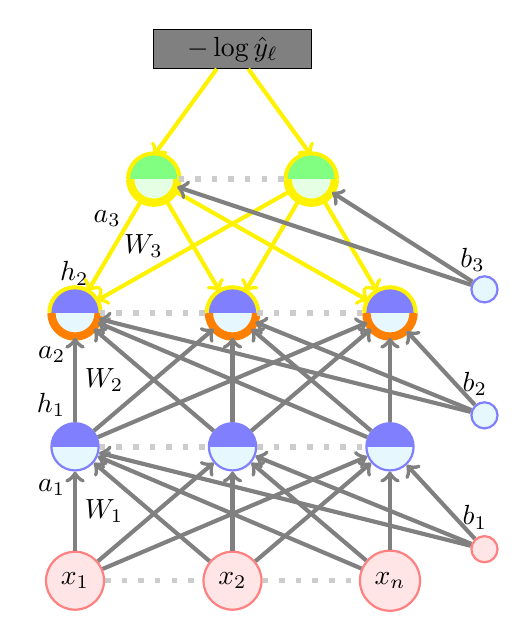
\begin{tikzpicture}
	\node [input_neuron] (neuron01) at (0,0) {$x_1$};
	\node [input_neuron] (neuron02) at (2,0){$x_2$};
	\node [input_neuron] (neuron03) at (4,0) {$x_n$};

	\node [bias_neuron] (neuron04) at (5.2,0.4) {};


	\node [hidden_neuron] (neuron11) at (0,1.7)  {};
	\node [hidden_neuron] (neuron12) at (2,1.7)  {};
	\node [hidden_neuron] (neuron13) at (4,1.7)  {};

	\node [bias_hidden_neuron] (neuron14) at (5.2,2.1) {};

	\begin{scope}
		\path[clip] (0,1.7) circle (3mm);
		\path[fill=blue!50] (-0.4,1.7) rectangle (0.3,2);
	\end{scope}
	\begin{scope}
		\path[clip] (2,1.7) circle (3mm);
		\path[fill=blue!50] (1.6,1.7) rectangle (2.3,2);
	\end{scope}
	\begin{scope}
		\path[clip] (4,1.7) circle (3mm);
		\path[fill=blue!50] (3.6,1.7) rectangle (4.3,2);
	\end{scope}


	\node [hidden_neuron] (neuron21) at (0,3.4)  {};
	\node [hidden_neuron] (neuron22) at (2,3.4)  {};
	\node [hidden_neuron] (neuron23) at (4,3.4)  {};

	\draw [yellow, line width = 3] (0.3,3.4) arc (0:180:3mm) {};
	\draw [yellow, line width = 3] (2.3,3.4) arc (0:180:3mm) {};
	\draw [yellow, line width = 3] (4.3,3.4) arc (0:180:3mm) {};

	\draw[orange, line width = 3] (-0.3, 3.4) arc (180:360:3mm){};
	\draw[orange, line width = 3] (1.7, 3.4) arc (180:360:3mm){};
	\draw[orange, line width = 3] (3.7, 3.4) arc (180:360:3mm){};
	\node [bias_hidden_neuron] (neuron24) at (5.2,3.7) {};


	\begin{scope}
		\path[clip] (0,3.4) circle (3mm);
		\path[fill=blue!50] (-0.4,3.4) rectangle (0.4,3.7);
	\end{scope}
	\begin{scope}
		\path[clip] (2,3.4) circle (3mm);
		\path[fill=blue!50] (1.6,3.4) rectangle (2.4,3.7);
	\end{scope}
	\begin{scope}
		\path[clip] (4,3.4) circle (3mm);
		\path[fill=blue!50] (3.6,3.4) rectangle (4.4,3.7);
	\end{scope}


	\node [output_neuron] (neuron31) at (1,5.1)  {};
	\node [output_neuron] (neuron32) at (3,5.1)  {};
	\draw [fill=gray] (1, 7) rectangle (3, 6.5) node[pos=0.5] {$-\log\hat{y}_\ell$};
	%\draw [black!50,line width=1.5pt,  ->] (1, 5.4) -- (1.8, 6.5);
	%\draw [black!50, line width=1.5pt, ->]  (3, 5.4) -- (2.2, 6.5);
	\draw [yellow,line width=1.5pt,  ->] (1.8, 6.5) -- (1, 5.4);
	\draw [yellow, line width=1.5pt, ->]  (2.2, 6.5) -- (3, 5.4);
	\draw [yellow, line width = 3] (1.3,5.1) arc (0:180:3mm) {};
	\draw [yellow, line width = 3] (3.3,5.1) arc (0:180:3mm) {};
	\draw[yellow, line width = 3] (0.7, 5.1) arc (180:360:3mm){};
	\draw[yellow, line width = 3] (2.7, 5.1) arc (180:360:3mm){};


	\begin{scope}
		\path[clip] (1,5.1) circle (3mm);
		\path[fill=green!50] (0.6,5.1) rectangle (1.3,5.4);
	\end{scope}
	\begin{scope}
		\path[clip] (3,5.1) circle (3mm);
		\path[fill=green!50] (2.6,5.1) rectangle (3.3,5.4);
	\end{scope}

	\draw[white,->] (neuron01) -- (neuron11) node[black,pos=.5,right]  {$W_{1}$} node[black,pos=0.8,left] {$a_{1}$};

	\draw[white,->] (neuron11) -- (neuron21) node[black,pos=.5,right] {$W_{2}$} node[black,pos=0.8,left] {$a_{2}$} node[black,pos=.2,left] {$h_{1}$};
	\draw[white,->] (neuron21) -- (neuron31) node[black,pos=.5,right] {$W_{3}$} node[black,pos=0.8,left] {$a_{3}$} node[black,pos=.2,left] {$h_{2}$};

	\draw[white,->] (neuron04) -- (neuron13) node[black,pos=0,right,above] {$b_1$};

	\draw[white,->] (neuron14) -- (neuron23) node[black,pos=0,right,above] {$b_2$};

	\draw[white,->] (neuron24) -- (neuron32) node[black,pos=0,right,above] {$b_3$};


	%\draw[white,->] (neuron31) -- (2.4.9) node[black,pos=1,above] {y };
	%\draw[white,->] (neuron31) -- (3,6.5) node[black,pos=1,above] {$f(x)$};
	%node[pos=1.3,above,right] {$\mathscr{L}(\theta)$};

	\draw[black!20,line width=2pt,loosely dotted] (neuron01) -- (neuron02);
	\draw[black!20,line width=2pt,loosely dotted] (neuron02) -- (neuron03);
	\draw[black!20,line width=2pt,loosely dotted] (neuron11) -- (neuron12);
	\draw[black!20,line width=2pt,loosely dotted] (neuron12) -- (neuron13);
	\draw[black!20,line width=2pt,loosely dotted] (neuron21) -- (neuron22);
	\draw[black!20,line width=2pt,loosely dotted] (neuron22) -- (neuron23);
	\draw[black!20,line width=2pt,loosely dotted] (neuron31) -- (neuron32);


	\foreach \from in {neuron01,neuron02,neuron03,neuron04}
	\foreach \to in {neuron11,neuron12,neuron13}
	\draw [black!50,line width=1.5pt,->] (\from) -- (\to);

	\foreach \from in {neuron11,neuron12,neuron13,neuron14}
	\foreach \to in {neuron21,neuron22,neuron23}
	\draw [black!50,line width=1.5pt,->] (\from) -- (\to);

	\foreach \from in {neuron21,neuron22,neuron23}
	\foreach \to in {neuron31,neuron32}
	\draw [yellow,line width=1.5pt,->] (\to) -- (\from);

	\draw [black!50,line width=1.5pt,->] (neuron24) -- (neuron31);
	\draw [black!50,line width=1.5pt,->] (neuron24) -- (neuron32);

\end{tikzpicture}
}
\savestack{\nnhiddencomp}{\hspace{-0.1in}
\tikzstyle{input_neuron}=[circle,draw=red!50,fill=red!10,thick,minimum size=5mm]
\tikzstyle{hidden_neuron}=[circle,draw=blue!50,fill=cyan!10,thick,minimum size=6mm]
\tikzstyle{output_neuron}=[circle,draw=green!50,fill=green!10,thick,minimum size=6mm]
\tikzstyle{bias_neuron}=[circle,draw=red!50,fill=red!10,thick,minimum size=2mm]
\tikzstyle{bias_hidden_neuron}=[circle,draw=blue!50,fill=cyan!10,thick,minimum size=2mm]

\tikzstyle{input}=[circle,draw=black!50,fill=black!20,thick,minimum size=6mm]

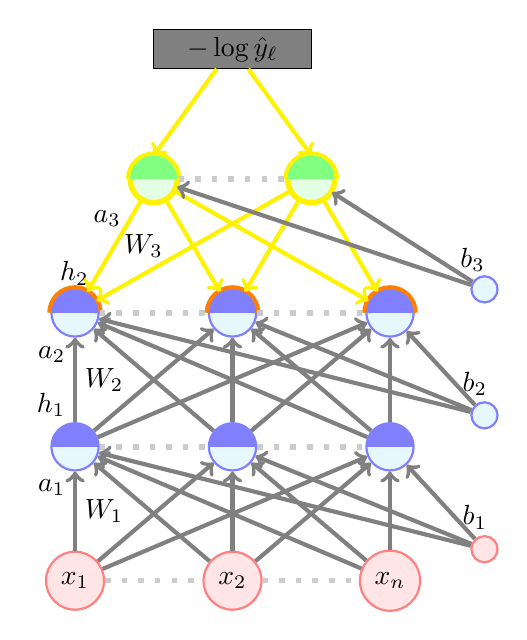
\begin{tikzpicture}
	\node [input_neuron] (neuron01) at (0,0) {$x_1$};
	\node [input_neuron] (neuron02) at (2,0){$x_2$};
	\node [input_neuron] (neuron03) at (4,0) {$x_n$};

	\node [bias_neuron] (neuron04) at (5.2,0.4) {};


	\node [hidden_neuron] (neuron11) at (0,1.7)  {};
	\node [hidden_neuron] (neuron12) at (2,1.7)  {};
	\node [hidden_neuron] (neuron13) at (4,1.7)  {};

	\node [bias_hidden_neuron] (neuron14) at (5.2,2.1) {};

	\begin{scope}
		\path[clip] (0,1.7) circle (3mm);
		\path[fill=blue!50] (-0.4,1.7) rectangle (0.3,2);
	\end{scope}
	\begin{scope}
		\path[clip] (2,1.7) circle (3mm);
		\path[fill=blue!50] (1.6,1.7) rectangle (2.3,2);
	\end{scope}
	\begin{scope}
		\path[clip] (4,1.7) circle (3mm);
		\path[fill=blue!50] (3.6,1.7) rectangle (4.3,2);
	\end{scope}


	\node [hidden_neuron] (neuron21) at (0,3.4)  {};
	\node [hidden_neuron] (neuron22) at (2,3.4)  {};
	\node [hidden_neuron] (neuron23) at (4,3.4)  {};

	\draw [orange, line width = 3] (0.3,3.4) arc (0:180:3mm) {};
	\draw [orange, line width = 3] (2.3,3.4) arc (0:180:3mm) {};
	\draw [orange, line width = 3] (4.3,3.4) arc (0:180:3mm) {};
	\node [bias_hidden_neuron] (neuron24) at (5.2,3.7) {};


	\begin{scope}
		\path[clip] (0,3.4) circle (3mm);
		\path[fill=blue!50] (-0.4,3.4) rectangle (0.4,3.7);
	\end{scope}
	\begin{scope}
		\path[clip] (2,3.4) circle (3mm);
		\path[fill=blue!50] (1.6,3.4) rectangle (2.4,3.7);
	\end{scope}
	\begin{scope}
		\path[clip] (4,3.4) circle (3mm);
		\path[fill=blue!50] (3.6,3.4) rectangle (4.4,3.7);
	\end{scope}


	\node [output_neuron] (neuron31) at (1,5.1)  {};
	\node [output_neuron] (neuron32) at (3,5.1)  {};
	\draw [fill=gray] (1, 7) rectangle (3, 6.5) node[pos=0.5] {$-\log\hat{y}_\ell$};
	%\draw [black!50,line width=1.5pt,  ->] (1, 5.4) -- (1.8, 6.5);
	%\draw [black!50, line width=1.5pt, ->]  (3, 5.4) -- (2.2, 6.5);
	\draw [yellow,line width=1.5pt,  ->] (1.8, 6.5) -- (1, 5.4);
	\draw [yellow, line width=1.5pt, ->]  (2.2, 6.5) -- (3, 5.4);
	\draw [yellow, line width = 3] (1.3,5.1) arc (0:180:3mm) {};
	\draw [yellow, line width = 3] (3.3,5.1) arc (0:180:3mm) {};
	\draw[yellow, line width = 2] (0.7, 5.1) arc (180:360:3mm){};
	\draw[yellow, line width = 2] (2.7, 5.1) arc (180:360:3mm){};


	\begin{scope}
		\path[clip] (1,5.1) circle (3mm);
		\path[fill=green!50] (0.6,5.1) rectangle (1.3,5.4);
	\end{scope}
	\begin{scope}
		\path[clip] (3,5.1) circle (3mm);
		\path[fill=green!50] (2.6,5.1) rectangle (3.3,5.4);
	\end{scope}

	\draw[white,->] (neuron01) -- (neuron11) node[black,pos=.5,right]  {$W_{1}$} node[black,pos=0.8,left] {$a_{1}$};

	\draw[white,->] (neuron11) -- (neuron21) node[black,pos=.5,right] {$W_{2}$} node[black,pos=0.8,left] {$a_{2}$} node[black,pos=.2,left] {$h_{1}$};
	\draw[white,->] (neuron21) -- (neuron31) node[black,pos=.5,right] {$W_{3}$} node[black,pos=0.8,left] {$a_{3}$} node[black,pos=.2,left] {$h_{2}$};

	\draw[white,->] (neuron04) -- (neuron13) node[black,pos=0,right,above] {$b_1$};

	\draw[white,->] (neuron14) -- (neuron23) node[black,pos=0,right,above] {$b_2$};

	\draw[white,->] (neuron24) -- (neuron32) node[black,pos=0,right,above] {$b_3$};


	%\draw[white,->] (neuron31) -- (2.4.9) node[black,pos=1,above] {y };
	%\draw[white,->] (neuron31) -- (3,6.5) node[black,pos=1,above] {$f(x)$};
	%node[pos=1.3,above,right] {$\mathscr{L}(\theta)$};

	\draw[black!20,line width=2pt,loosely dotted] (neuron01) -- (neuron02);
	\draw[black!20,line width=2pt,loosely dotted] (neuron02) -- (neuron03);
	\draw[black!20,line width=2pt,loosely dotted] (neuron11) -- (neuron12);
	\draw[black!20,line width=2pt,loosely dotted] (neuron12) -- (neuron13);
	\draw[black!20,line width=2pt,loosely dotted] (neuron21) -- (neuron22);
	\draw[black!20,line width=2pt,loosely dotted] (neuron22) -- (neuron23);
	\draw[black!20,line width=2pt,loosely dotted] (neuron31) -- (neuron32);


	\foreach \from in {neuron01,neuron02,neuron03,neuron04}
	\foreach \to in {neuron11,neuron12,neuron13}
	\draw [black!50,line width=1.5pt,->] (\from) -- (\to);

	\foreach \from in {neuron11,neuron12,neuron13,neuron14}
	\foreach \to in {neuron21,neuron22,neuron23}
	\draw [black!50,line width=1.5pt,->] (\from) -- (\to);

	\foreach \from in {neuron21,neuron22,neuron23}
	\foreach \to in {neuron31,neuron32}
	\draw [yellow,line width=1.5pt,->] (\to) -- (\from);

	\draw [black!50,line width=1.5pt,->] (neuron24) -- (neuron31);
	\draw [black!50,line width=1.5pt,->] (neuron24) -- (neuron32);

\end{tikzpicture}
}
\savestack{\nnhiddensimp}{\hspace{-0.1in}
\tikzstyle{input_neuron}=[circle,draw=red!50,fill=red!10,thick,minimum size=5mm]
\tikzstyle{hidden_neuron}=[circle,draw=blue!50,fill=cyan!10,thick,minimum size=6mm]
\tikzstyle{output_neuron}=[circle,draw=green!50,fill=green!10,thick,minimum size=6mm]
\tikzstyle{bias_neuron}=[circle,draw=red!50,fill=red!10,thick,minimum size=2mm]
\tikzstyle{bias_hidden_neuron}=[circle,draw=blue!50,fill=cyan!10,thick,minimum size=2mm]

\tikzstyle{input}=[circle,draw=black!50,fill=black!20,thick,minimum size=6mm]

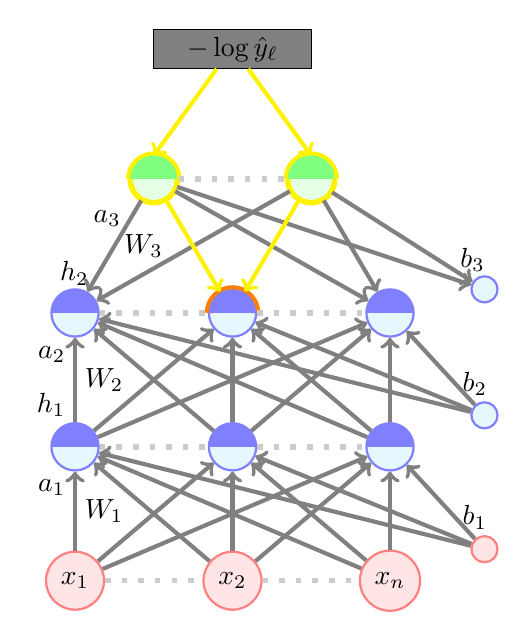
\begin{tikzpicture}


	\node [input_neuron] (neuron01) at (0,0) {$x_1$};
	\node [input_neuron] (neuron02) at (2,0){$x_2$};
	\node [input_neuron] (neuron03) at (4,0) {$x_n$};

	\node [bias_neuron] (neuron04) at (5.2,0.4) {};


	\node [hidden_neuron] (neuron11) at (0,1.7)  {};
	\node [hidden_neuron] (neuron12) at (2,1.7)  {};
	\node [hidden_neuron] (neuron13) at (4,1.7)  {};

	\node [bias_hidden_neuron] (neuron14) at (5.2,2.1) {};

	\begin{scope}
		\path[clip] (0,1.7) circle (3mm);
		\path[fill=blue!50] (-0.4,1.7) rectangle (0.3,2);
	\end{scope}
	\begin{scope}
		\path[clip] (2,1.7) circle (3mm);
		\path[fill=blue!50] (1.6,1.7) rectangle (2.3,2);
	\end{scope}
	\begin{scope}
		\path[clip] (4,1.7) circle (3mm);
		\path[fill=blue!50] (3.6,1.7) rectangle (4.3,2);
	\end{scope}


	\node [hidden_neuron] (neuron21) at (0,3.4)  {};
	\node [hidden_neuron] (neuron22) at (2,3.4)  {};
	\node [hidden_neuron] (neuron23) at (4,3.4)  {};

	\draw [orange, line width = 3] (2.3,3.4) arc (0:180:3mm) {};
	\node [bias_hidden_neuron] (neuron24) at (5.2,3.7) {};


	\begin{scope}
		\path[clip] (0,3.4) circle (3mm);
		\path[fill=blue!50] (-0.4,3.4) rectangle (0.4,3.7);
	\end{scope}
	\begin{scope}
		\path[clip] (2,3.4) circle (3mm);
		\path[fill=blue!50] (1.6,3.4) rectangle (2.4,3.7);
	\end{scope}
	\begin{scope}
		\path[clip] (4,3.4) circle (3mm);
		\path[fill=blue!50] (3.6,3.4) rectangle (4.4,3.7);
	\end{scope}


	\node [output_neuron] (neuron31) at (1,5.1)  {};
	\node [output_neuron] (neuron32) at (3,5.1)  {};
	\draw [fill=gray] (1, 7) rectangle (3, 6.5) node[pos=0.5] {$-\log\hat{y}_\ell$};
	%\draw [black!50,line width=1.5pt,  ->] (1, 5.4) -- (1.8, 6.5);
	%\draw [black!50, line width=1.5pt, ->]  (3, 5.4) -- (2.2, 6.5);
	\draw [yellow,line width=1.5pt,  ->] (1.8, 6.5) -- (1, 5.4);
	\draw [yellow, line width=1.5pt, ->]  (2.2, 6.5) -- (3, 5.4);
	\draw [yellow, line width = 3] (1.3,5.1) arc (0:180:3mm) {};
	\draw [yellow, line width = 3] (3.3,5.1) arc (0:180:3mm) {};
	\draw[yellow, line width = 2] (0.7, 5.1) arc (180:360:3mm){};
	\draw[yellow, line width = 2] (2.7, 5.1) arc (180:360:3mm){};


	\begin{scope}
		\path[clip] (1,5.1) circle (3mm);
		\path[fill=green!50] (0.6,5.1) rectangle (1.3,5.4);
	\end{scope}
	\begin{scope}
		\path[clip] (3,5.1) circle (3mm);
		\path[fill=green!50] (2.6,5.1) rectangle (3.3,5.4);
	\end{scope}

	\draw[white,->] (neuron01) -- (neuron11) node[black,pos=.5,right]  {$W_{1}$} node[black,pos=0.8,left] {$a_{1}$};

	\draw[white,->] (neuron11) -- (neuron21) node[black,pos=.5,right] {$W_{2}$} node[black,pos=0.8,left] {$a_{2}$} node[black,pos=.2,left] {$h_{1}$};
	\draw[white,->] (neuron21) -- (neuron31) node[black,pos=.5,right] {$W_{3}$} node[black,pos=0.8,left] {$a_{3}$} node[black,pos=.2,left] {$h_{2}$};

	\draw[white,->] (neuron04) -- (neuron13) node[black,pos=0,right,above] {$b_1$};

	\draw[white,->] (neuron14) -- (neuron23) node[black,pos=0,right,above] {$b_2$};

	\draw[white,->] (neuron24) -- (neuron32) node[black,pos=0,right,above] {$b_3$};


	%\draw[white,->] (neuron31) -- (2.4.9) node[black,pos=1,above] {y };
	%\draw[white,->] (neuron31) -- (3,6.5) node[black,pos=1,above] {$f(x)$};
	%node[pos=1.3,above,right] {$\mathscr{L}(\theta)$};

	\draw[black!20,line width=2pt,loosely dotted] (neuron01) -- (neuron02);
	\draw[black!20,line width=2pt,loosely dotted] (neuron02) -- (neuron03);
	\draw[black!20,line width=2pt,loosely dotted] (neuron11) -- (neuron12);
	\draw[black!20,line width=2pt,loosely dotted] (neuron12) -- (neuron13);
	\draw[black!20,line width=2pt,loosely dotted] (neuron21) -- (neuron22);
	\draw[black!20,line width=2pt,loosely dotted] (neuron22) -- (neuron23);
	\draw[black!20,line width=2pt,loosely dotted] (neuron31) -- (neuron32);


	\foreach \from in {neuron01,neuron02,neuron03,neuron04}
	\foreach \to in {neuron11,neuron12,neuron13}
	\draw [black!50,line width=1.5pt,->] (\from) -- (\to);

	\foreach \from in {neuron11,neuron12,neuron13,neuron14}
	\foreach \to in {neuron21,neuron22,neuron23}
	\draw [black!50,line width=1.5pt,->] (\from) -- (\to);

	\foreach \from in {neuron21,neuron24,neuron23}
	\foreach \to in {neuron31,neuron32}
	\draw [black!50,line width=1.5pt,->] (\to) -- (\from);

	\draw [yellow,line width=1.5pt,->]  (neuron31)--(neuron22);
	\draw [yellow,line width=1.5pt,->]  (neuron32)--(neuron22);

\end{tikzpicture}
}

\begin{frame}
  \myheading{Module 4.6: Backpropagation: Computing Gradients w.r.t. Hidden Units}
\end{frame}

%Slide 31
\begin{frame}
  \begin{overlayarea}{\textwidth}{\textheight}
    \textbf{Quantities of interest (roadmap for the remaining part):}
    \begin{itemize}
      % \justifying
      \item Gradient w.r.t. output units
      \item \alert<1->{Gradient w.r.t. hidden units}
      \item Gradient w.r.t. weights and biases
    \end{itemize}

    \begin{align*}
      \underbrace{\frac{\partial \mathscr{L}(\theta)}{\partial W_{11}}}_
      {\substack{\text{Talk to the}\\ \text{weight directly}}}
      =
      \underbrace{\frac{\partial \mathscr{L}(\theta)}{\partial \hat{y}} \frac{\partial \hat{y}}{\partial a_{3}}}_
        {\substack{\text{Talk to the} \\ \text{output layer}}}
      \alert<1->{\underbrace{\frac{\partial a_{3}}{\partial h_{2}} \frac{\partial h_{2}}{\partial a_{2}}}_
        {\substack{\text{Talk to the} \\ \text{previous hidden} \\ \text{layer}}}
        \underbrace{\frac{\partial a_{2}}{\partial h_{1}} \frac{\partial h_{1}}{\partial a_{1}}}_
        {\substack{\text{Talk to the} \\ \text{previous} \\ \text{hidden layer}}}}
      \underbrace{\frac{\partial a_{1}}{\partial W_{11}}}_
      {\substack{\text{and now} \\ \text{talk to} \\ \text{the} \\ \text{weights}}}
    \end{align*}

    \begin{itemize}
      % \justifying
      \item<1-> Our focus is on \textit{Cross entropy loss} and \textit{Softmax} output.
    \end{itemize}
  \end{overlayarea}
\end{frame}

%Slide 32
\begin{frame}
  \begin{columns}
    \column{0.55\textwidth}
    \begin{overlayarea}{\textwidth}{\textheight}%\begin{block}{}
      % \justifying
      \textbf{Chain rule along multiple paths:} If a function $p(z)$ can be written as a function of intermediate results $q_i(z)$ then we have :

      \visible<2->{
        \begin{align*}
          \frac{\partial p(z)}{\partial z} & =
          \mathlarger{\sum_m} \frac{\partial p(z)}{\partial q_m(z)} \frac{\partial q_m(z)}{\partial z}
        \end{align*}
      }

      \visible<3->{
        In our case:
        \begin{itemize}
          % \justifying
          \item<3->$p(z)$ is the loss function $\mathscr{L}(\theta)$
          \item<4->$z = h_{ij}$
          \item<5->$q_m(z) = a_{Lm}$
        \end{itemize}
      }
    \end{overlayarea}
    \column{0.45\textwidth}
    \begin{overlayarea}{\textwidth}{\textheight}
      \makebox[\textwidth][c]{\usebox{\nnhiddensimpcontent}}
    \end{overlayarea}
    % \hspace{-0.1in}
\tikzstyle{input_neuron}=[circle,draw=red!50,fill=red!10,thick,minimum size=5mm]
\tikzstyle{hidden_neuron}=[circle,draw=blue!50,fill=cyan!10,thick,minimum size=6mm]
\tikzstyle{output_neuron}=[circle,draw=green!50,fill=green!10,thick,minimum size=6mm]
\tikzstyle{bias_neuron}=[circle,draw=red!50,fill=red!10,thick,minimum size=2mm]
\tikzstyle{bias_hidden_neuron}=[circle,draw=blue!50,fill=cyan!10,thick,minimum size=2mm]

\tikzstyle{input}=[circle,draw=black!50,fill=black!20,thick,minimum size=6mm]

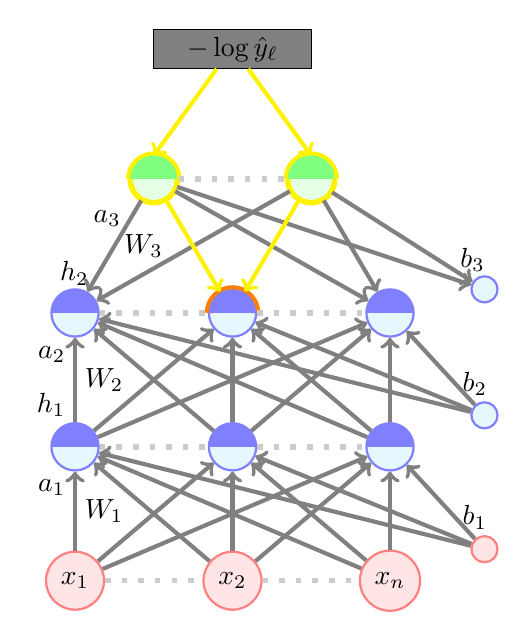
\begin{tikzpicture}


	\node [input_neuron] (neuron01) at (0,0) {$x_1$};
	\node [input_neuron] (neuron02) at (2,0){$x_2$};
	\node [input_neuron] (neuron03) at (4,0) {$x_n$};

	\node [bias_neuron] (neuron04) at (5.2,0.4) {};


	\node [hidden_neuron] (neuron11) at (0,1.7)  {};
	\node [hidden_neuron] (neuron12) at (2,1.7)  {};
	\node [hidden_neuron] (neuron13) at (4,1.7)  {};

	\node [bias_hidden_neuron] (neuron14) at (5.2,2.1) {};

	\begin{scope}
		\path[clip] (0,1.7) circle (3mm);
		\path[fill=blue!50] (-0.4,1.7) rectangle (0.3,2);
	\end{scope}
	\begin{scope}
		\path[clip] (2,1.7) circle (3mm);
		\path[fill=blue!50] (1.6,1.7) rectangle (2.3,2);
	\end{scope}
	\begin{scope}
		\path[clip] (4,1.7) circle (3mm);
		\path[fill=blue!50] (3.6,1.7) rectangle (4.3,2);
	\end{scope}


	\node [hidden_neuron] (neuron21) at (0,3.4)  {};
	\node [hidden_neuron] (neuron22) at (2,3.4)  {};
	\node [hidden_neuron] (neuron23) at (4,3.4)  {};

	\draw [orange, line width = 3] (2.3,3.4) arc (0:180:3mm) {};
	\node [bias_hidden_neuron] (neuron24) at (5.2,3.7) {};


	\begin{scope}
		\path[clip] (0,3.4) circle (3mm);
		\path[fill=blue!50] (-0.4,3.4) rectangle (0.4,3.7);
	\end{scope}
	\begin{scope}
		\path[clip] (2,3.4) circle (3mm);
		\path[fill=blue!50] (1.6,3.4) rectangle (2.4,3.7);
	\end{scope}
	\begin{scope}
		\path[clip] (4,3.4) circle (3mm);
		\path[fill=blue!50] (3.6,3.4) rectangle (4.4,3.7);
	\end{scope}


	\node [output_neuron] (neuron31) at (1,5.1)  {};
	\node [output_neuron] (neuron32) at (3,5.1)  {};
	\draw [fill=gray] (1, 7) rectangle (3, 6.5) node[pos=0.5] {$-\log\hat{y}_\ell$};
	%\draw [black!50,line width=1.5pt,  ->] (1, 5.4) -- (1.8, 6.5);
	%\draw [black!50, line width=1.5pt, ->]  (3, 5.4) -- (2.2, 6.5);
	\draw [yellow,line width=1.5pt,  ->] (1.8, 6.5) -- (1, 5.4);
	\draw [yellow, line width=1.5pt, ->]  (2.2, 6.5) -- (3, 5.4);
	\draw [yellow, line width = 3] (1.3,5.1) arc (0:180:3mm) {};
	\draw [yellow, line width = 3] (3.3,5.1) arc (0:180:3mm) {};
	\draw[yellow, line width = 2] (0.7, 5.1) arc (180:360:3mm){};
	\draw[yellow, line width = 2] (2.7, 5.1) arc (180:360:3mm){};


	\begin{scope}
		\path[clip] (1,5.1) circle (3mm);
		\path[fill=green!50] (0.6,5.1) rectangle (1.3,5.4);
	\end{scope}
	\begin{scope}
		\path[clip] (3,5.1) circle (3mm);
		\path[fill=green!50] (2.6,5.1) rectangle (3.3,5.4);
	\end{scope}

	\draw[white,->] (neuron01) -- (neuron11) node[black,pos=.5,right]  {$W_{1}$} node[black,pos=0.8,left] {$a_{1}$};

	\draw[white,->] (neuron11) -- (neuron21) node[black,pos=.5,right] {$W_{2}$} node[black,pos=0.8,left] {$a_{2}$} node[black,pos=.2,left] {$h_{1}$};
	\draw[white,->] (neuron21) -- (neuron31) node[black,pos=.5,right] {$W_{3}$} node[black,pos=0.8,left] {$a_{3}$} node[black,pos=.2,left] {$h_{2}$};

	\draw[white,->] (neuron04) -- (neuron13) node[black,pos=0,right,above] {$b_1$};

	\draw[white,->] (neuron14) -- (neuron23) node[black,pos=0,right,above] {$b_2$};

	\draw[white,->] (neuron24) -- (neuron32) node[black,pos=0,right,above] {$b_3$};


	%\draw[white,->] (neuron31) -- (2.4.9) node[black,pos=1,above] {y };
	%\draw[white,->] (neuron31) -- (3,6.5) node[black,pos=1,above] {$f(x)$};
	%node[pos=1.3,above,right] {$\mathscr{L}(\theta)$};

	\draw[black!20,line width=2pt,loosely dotted] (neuron01) -- (neuron02);
	\draw[black!20,line width=2pt,loosely dotted] (neuron02) -- (neuron03);
	\draw[black!20,line width=2pt,loosely dotted] (neuron11) -- (neuron12);
	\draw[black!20,line width=2pt,loosely dotted] (neuron12) -- (neuron13);
	\draw[black!20,line width=2pt,loosely dotted] (neuron21) -- (neuron22);
	\draw[black!20,line width=2pt,loosely dotted] (neuron22) -- (neuron23);
	\draw[black!20,line width=2pt,loosely dotted] (neuron31) -- (neuron32);


	\foreach \from in {neuron01,neuron02,neuron03,neuron04}
	\foreach \to in {neuron11,neuron12,neuron13}
	\draw [black!50,line width=1.5pt,->] (\from) -- (\to);

	\foreach \from in {neuron11,neuron12,neuron13,neuron14}
	\foreach \to in {neuron21,neuron22,neuron23}
	\draw [black!50,line width=1.5pt,->] (\from) -- (\to);

	\foreach \from in {neuron21,neuron24,neuron23}
	\foreach \to in {neuron31,neuron32}
	\draw [black!50,line width=1.5pt,->] (\to) -- (\from);

	\draw [yellow,line width=1.5pt,->]  (neuron31)--(neuron22);
	\draw [yellow,line width=1.5pt,->]  (neuron32)--(neuron22);

\end{tikzpicture}

  \end{columns}
\end{frame}

\begin{frame}[b]
    \visible<1>{\tiny Intentionally left blank}
\end{frame}

%Slide 33
\begin{frame}
  \begin{columns}
    \column{0.55\textwidth}
    \begin{overlayarea}{\textwidth}{\textheight}
      \begin{itemize}[]
      % \justifying
        \item[] $\frac{\partial \mathscr{L}(\theta)}{\partial h_{ij}} \visible<2->{ =
                \mathlarger{\sum_{m=1}^{k}} \frac{\partial \mathscr{L}(\theta)}{\partial a_{i+1, m}} \frac{\partial a_{i+1, m}}{\partial h_{ij}}}$
        \item[]<3-> $\hspace{1cm}= \mathlarger{\sum_{m= 1}^{k}} \frac{\partial \mathscr{L}(\theta)}{\partial a_{i+1, m}} W_{i+1,m,j}$
      \end{itemize}
      \visible<4->{Now consider these two vectors,}
      \begin{align*}
        \visible<5-> {\nabla_{a_{i+1}} \mathscr{L}(\theta) =
        \begin{bmatrix}
            % Need to change this on clarification
            \visible<6->{\frac{\partial \mathscr{L}(\theta)}{\partial a_{i+1,1} }}  \\
            \visible<8->{\vdots}                                                    \\
            \visible<9->{\frac{\partial \mathscr{L}(\theta)}{\partial a_{i+1,k}}}
          \end{bmatrix}; \visible<5->{W_{i+1,\hspace{0.025in}\cdot\hspace{0.025in}, j}} = \begin{bmatrix}
            \visible<7->{ W_{i+1,1,j}}   \\
            \visible<8->{\vdots}         \\
            \visible<10->{W_{i+1,k,j}}
          \end{bmatrix}}
      \end{align*}
      \visible<12->{$W_{i+1,\hspace{0.025in}\cdot\hspace{0.025in}, j}$ is the $j$-th column of $W_{i+1}$; \visible<13->{see that,}}
      \begin{align*}
        \visible<14-> {(W_{i+1,\hspace{0.025in}\cdot\hspace{0.025in}, j})^T \nabla_{a_{i+1}} \mathscr{L}(\theta) =} \visible<15->{\mathlarger{\sum_{m=1}^{k}} \frac{\partial \mathscr{L}(\theta)}{\partial a_{i+1, m}} W_{i+1,m,j} }
      \end{align*}
    \end{overlayarea}
    \column{0.45\textwidth}
    \begin{overlayarea}{\textwidth}{\textheight}
      \makebox[\textwidth][c]{\usebox{\nnhiddensimpcontent}}
      \begin{center}
        $a_{i+1} = W_{i+1}h_{ij}+b_{i+1}$
      \end{center}
    \end{overlayarea}
    % \hspace{-0.1in}
\tikzstyle{input_neuron}=[circle,draw=red!50,fill=red!10,thick,minimum size=5mm]
\tikzstyle{hidden_neuron}=[circle,draw=blue!50,fill=cyan!10,thick,minimum size=6mm]
\tikzstyle{output_neuron}=[circle,draw=green!50,fill=green!10,thick,minimum size=6mm]
\tikzstyle{bias_neuron}=[circle,draw=red!50,fill=red!10,thick,minimum size=2mm]
\tikzstyle{bias_hidden_neuron}=[circle,draw=blue!50,fill=cyan!10,thick,minimum size=2mm]

\tikzstyle{input}=[circle,draw=black!50,fill=black!20,thick,minimum size=6mm]

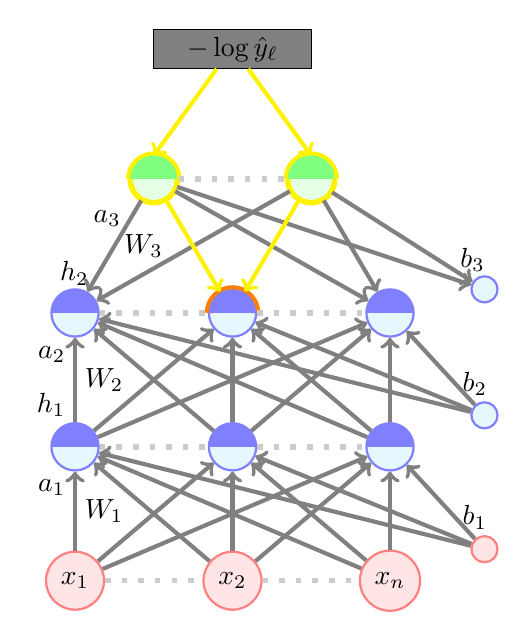
\begin{tikzpicture}


	\node [input_neuron] (neuron01) at (0,0) {$x_1$};
	\node [input_neuron] (neuron02) at (2,0){$x_2$};
	\node [input_neuron] (neuron03) at (4,0) {$x_n$};

	\node [bias_neuron] (neuron04) at (5.2,0.4) {};


	\node [hidden_neuron] (neuron11) at (0,1.7)  {};
	\node [hidden_neuron] (neuron12) at (2,1.7)  {};
	\node [hidden_neuron] (neuron13) at (4,1.7)  {};

	\node [bias_hidden_neuron] (neuron14) at (5.2,2.1) {};

	\begin{scope}
		\path[clip] (0,1.7) circle (3mm);
		\path[fill=blue!50] (-0.4,1.7) rectangle (0.3,2);
	\end{scope}
	\begin{scope}
		\path[clip] (2,1.7) circle (3mm);
		\path[fill=blue!50] (1.6,1.7) rectangle (2.3,2);
	\end{scope}
	\begin{scope}
		\path[clip] (4,1.7) circle (3mm);
		\path[fill=blue!50] (3.6,1.7) rectangle (4.3,2);
	\end{scope}


	\node [hidden_neuron] (neuron21) at (0,3.4)  {};
	\node [hidden_neuron] (neuron22) at (2,3.4)  {};
	\node [hidden_neuron] (neuron23) at (4,3.4)  {};

	\draw [orange, line width = 3] (2.3,3.4) arc (0:180:3mm) {};
	\node [bias_hidden_neuron] (neuron24) at (5.2,3.7) {};


	\begin{scope}
		\path[clip] (0,3.4) circle (3mm);
		\path[fill=blue!50] (-0.4,3.4) rectangle (0.4,3.7);
	\end{scope}
	\begin{scope}
		\path[clip] (2,3.4) circle (3mm);
		\path[fill=blue!50] (1.6,3.4) rectangle (2.4,3.7);
	\end{scope}
	\begin{scope}
		\path[clip] (4,3.4) circle (3mm);
		\path[fill=blue!50] (3.6,3.4) rectangle (4.4,3.7);
	\end{scope}


	\node [output_neuron] (neuron31) at (1,5.1)  {};
	\node [output_neuron] (neuron32) at (3,5.1)  {};
	\draw [fill=gray] (1, 7) rectangle (3, 6.5) node[pos=0.5] {$-\log\hat{y}_\ell$};
	%\draw [black!50,line width=1.5pt,  ->] (1, 5.4) -- (1.8, 6.5);
	%\draw [black!50, line width=1.5pt, ->]  (3, 5.4) -- (2.2, 6.5);
	\draw [yellow,line width=1.5pt,  ->] (1.8, 6.5) -- (1, 5.4);
	\draw [yellow, line width=1.5pt, ->]  (2.2, 6.5) -- (3, 5.4);
	\draw [yellow, line width = 3] (1.3,5.1) arc (0:180:3mm) {};
	\draw [yellow, line width = 3] (3.3,5.1) arc (0:180:3mm) {};
	\draw[yellow, line width = 2] (0.7, 5.1) arc (180:360:3mm){};
	\draw[yellow, line width = 2] (2.7, 5.1) arc (180:360:3mm){};


	\begin{scope}
		\path[clip] (1,5.1) circle (3mm);
		\path[fill=green!50] (0.6,5.1) rectangle (1.3,5.4);
	\end{scope}
	\begin{scope}
		\path[clip] (3,5.1) circle (3mm);
		\path[fill=green!50] (2.6,5.1) rectangle (3.3,5.4);
	\end{scope}

	\draw[white,->] (neuron01) -- (neuron11) node[black,pos=.5,right]  {$W_{1}$} node[black,pos=0.8,left] {$a_{1}$};

	\draw[white,->] (neuron11) -- (neuron21) node[black,pos=.5,right] {$W_{2}$} node[black,pos=0.8,left] {$a_{2}$} node[black,pos=.2,left] {$h_{1}$};
	\draw[white,->] (neuron21) -- (neuron31) node[black,pos=.5,right] {$W_{3}$} node[black,pos=0.8,left] {$a_{3}$} node[black,pos=.2,left] {$h_{2}$};

	\draw[white,->] (neuron04) -- (neuron13) node[black,pos=0,right,above] {$b_1$};

	\draw[white,->] (neuron14) -- (neuron23) node[black,pos=0,right,above] {$b_2$};

	\draw[white,->] (neuron24) -- (neuron32) node[black,pos=0,right,above] {$b_3$};


	%\draw[white,->] (neuron31) -- (2.4.9) node[black,pos=1,above] {y };
	%\draw[white,->] (neuron31) -- (3,6.5) node[black,pos=1,above] {$f(x)$};
	%node[pos=1.3,above,right] {$\mathscr{L}(\theta)$};

	\draw[black!20,line width=2pt,loosely dotted] (neuron01) -- (neuron02);
	\draw[black!20,line width=2pt,loosely dotted] (neuron02) -- (neuron03);
	\draw[black!20,line width=2pt,loosely dotted] (neuron11) -- (neuron12);
	\draw[black!20,line width=2pt,loosely dotted] (neuron12) -- (neuron13);
	\draw[black!20,line width=2pt,loosely dotted] (neuron21) -- (neuron22);
	\draw[black!20,line width=2pt,loosely dotted] (neuron22) -- (neuron23);
	\draw[black!20,line width=2pt,loosely dotted] (neuron31) -- (neuron32);


	\foreach \from in {neuron01,neuron02,neuron03,neuron04}
	\foreach \to in {neuron11,neuron12,neuron13}
	\draw [black!50,line width=1.5pt,->] (\from) -- (\to);

	\foreach \from in {neuron11,neuron12,neuron13,neuron14}
	\foreach \to in {neuron21,neuron22,neuron23}
	\draw [black!50,line width=1.5pt,->] (\from) -- (\to);

	\foreach \from in {neuron21,neuron24,neuron23}
	\foreach \to in {neuron31,neuron32}
	\draw [black!50,line width=1.5pt,->] (\to) -- (\from);

	\draw [yellow,line width=1.5pt,->]  (neuron31)--(neuron22);
	\draw [yellow,line width=1.5pt,->]  (neuron32)--(neuron22);

\end{tikzpicture}

  \end{columns}
\end{frame}

%Slide 34
\begin{frame}
  \begin{columns}
    \column{0.61\textwidth}
    \begin{overlayarea}{\textwidth}{\textheight}
      \begin{align*}
        \textit{We have,} \frac{\partial \mathscr{L}(\theta)}{\partial h_{ij}} & =  (W_{i+1,.,j})^T \nabla_{a_{i+1}} \mathscr{L}(\theta)
      \end{align*}
      \visible<2->{We can now write the gradient w.r.t. $h_i$}
      \begin{align*}
        \visible<2->{\nabla_{\mathbf{h_i}} \mathscr{L}(\theta)} \visible<3->{ & =
          \begin{bmatrix}
            % Need to change this on clarification
            \visible<4->{\frac{\partial \mathscr{L}(\theta)}{\partial h_{i1}}} \\
            \visible<6->{\frac{\partial \mathscr{L}(\theta)}{\partial h_{i2}}} \\
            \visible<8->{\vdots}                                               \\
            \visible<9->{\frac{\partial \mathscr{L}(\theta)}{\partial h_{in}}}
          \end{bmatrix} =
          \begin{bmatrix}
            % Need to change this on clarification
            \visible<5->{(W_{i+1,\hspace{0.025in}\cdot\hspace{0.025in}, 1})^T \nabla_{a_{i+1}} \mathscr{L}(\theta)}  \\
            \visible<7->{(W_{i+1,\hspace{0.025in}\cdot\hspace{0.025in}, 2})^T \nabla_{a_{i+1}} \mathscr{L}(\theta)}  \\
            \visible<8->{\vdots}                                                                                     \\
            \visible<10->{(W_{i+1,\hspace{0.025in}\cdot\hspace{0.025in}, n})^T \nabla_{a_{i+1}} \mathscr{L}(\theta)}
          \end{bmatrix}} \\
        \visible<11->{                                          & = (W_{i+1})^T (\nabla_{a_{i+1}} \mathscr{L}(\theta))}
      \end{align*}

      \begin{itemize}
        % \justifying
        \item<12-> We are almost done except that we do not know how to calculate $\nabla_{a_{i+1}} \mathscr{L}(\theta)$ for $i < L-1$
        \item<13-> We will see how to compute that
      \end{itemize}
    \end{overlayarea}
    \column{0.39\textwidth}
    \begin{overlayarea}{\textwidth}{\textheight}
      \makebox[\textwidth][c]{\usebox{\nnhiddencompcontent}}
    \end{overlayarea}
    %   \hspace{-0.1in}
\tikzstyle{input_neuron}=[circle,draw=red!50,fill=red!10,thick,minimum size=5mm]
\tikzstyle{hidden_neuron}=[circle,draw=blue!50,fill=cyan!10,thick,minimum size=6mm]
\tikzstyle{output_neuron}=[circle,draw=green!50,fill=green!10,thick,minimum size=6mm]
\tikzstyle{bias_neuron}=[circle,draw=red!50,fill=red!10,thick,minimum size=2mm]
\tikzstyle{bias_hidden_neuron}=[circle,draw=blue!50,fill=cyan!10,thick,minimum size=2mm]

\tikzstyle{input}=[circle,draw=black!50,fill=black!20,thick,minimum size=6mm]

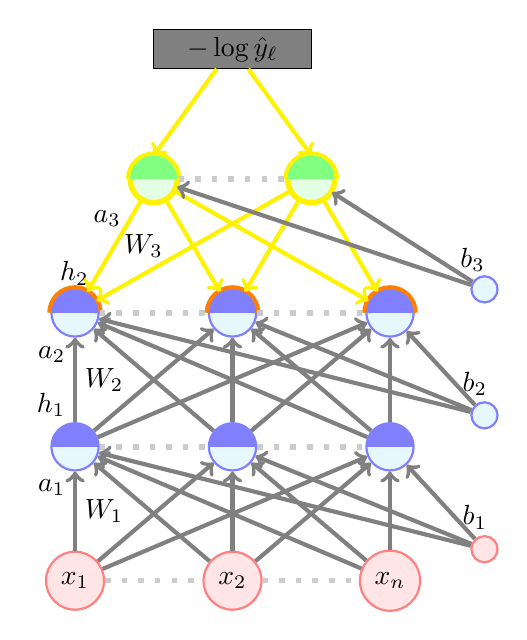
\begin{tikzpicture}
	\node [input_neuron] (neuron01) at (0,0) {$x_1$};
	\node [input_neuron] (neuron02) at (2,0){$x_2$};
	\node [input_neuron] (neuron03) at (4,0) {$x_n$};

	\node [bias_neuron] (neuron04) at (5.2,0.4) {};


	\node [hidden_neuron] (neuron11) at (0,1.7)  {};
	\node [hidden_neuron] (neuron12) at (2,1.7)  {};
	\node [hidden_neuron] (neuron13) at (4,1.7)  {};

	\node [bias_hidden_neuron] (neuron14) at (5.2,2.1) {};

	\begin{scope}
		\path[clip] (0,1.7) circle (3mm);
		\path[fill=blue!50] (-0.4,1.7) rectangle (0.3,2);
	\end{scope}
	\begin{scope}
		\path[clip] (2,1.7) circle (3mm);
		\path[fill=blue!50] (1.6,1.7) rectangle (2.3,2);
	\end{scope}
	\begin{scope}
		\path[clip] (4,1.7) circle (3mm);
		\path[fill=blue!50] (3.6,1.7) rectangle (4.3,2);
	\end{scope}


	\node [hidden_neuron] (neuron21) at (0,3.4)  {};
	\node [hidden_neuron] (neuron22) at (2,3.4)  {};
	\node [hidden_neuron] (neuron23) at (4,3.4)  {};

	\draw [orange, line width = 3] (0.3,3.4) arc (0:180:3mm) {};
	\draw [orange, line width = 3] (2.3,3.4) arc (0:180:3mm) {};
	\draw [orange, line width = 3] (4.3,3.4) arc (0:180:3mm) {};
	\node [bias_hidden_neuron] (neuron24) at (5.2,3.7) {};


	\begin{scope}
		\path[clip] (0,3.4) circle (3mm);
		\path[fill=blue!50] (-0.4,3.4) rectangle (0.4,3.7);
	\end{scope}
	\begin{scope}
		\path[clip] (2,3.4) circle (3mm);
		\path[fill=blue!50] (1.6,3.4) rectangle (2.4,3.7);
	\end{scope}
	\begin{scope}
		\path[clip] (4,3.4) circle (3mm);
		\path[fill=blue!50] (3.6,3.4) rectangle (4.4,3.7);
	\end{scope}


	\node [output_neuron] (neuron31) at (1,5.1)  {};
	\node [output_neuron] (neuron32) at (3,5.1)  {};
	\draw [fill=gray] (1, 7) rectangle (3, 6.5) node[pos=0.5] {$-\log\hat{y}_\ell$};
	%\draw [black!50,line width=1.5pt,  ->] (1, 5.4) -- (1.8, 6.5);
	%\draw [black!50, line width=1.5pt, ->]  (3, 5.4) -- (2.2, 6.5);
	\draw [yellow,line width=1.5pt,  ->] (1.8, 6.5) -- (1, 5.4);
	\draw [yellow, line width=1.5pt, ->]  (2.2, 6.5) -- (3, 5.4);
	\draw [yellow, line width = 3] (1.3,5.1) arc (0:180:3mm) {};
	\draw [yellow, line width = 3] (3.3,5.1) arc (0:180:3mm) {};
	\draw[yellow, line width = 2] (0.7, 5.1) arc (180:360:3mm){};
	\draw[yellow, line width = 2] (2.7, 5.1) arc (180:360:3mm){};


	\begin{scope}
		\path[clip] (1,5.1) circle (3mm);
		\path[fill=green!50] (0.6,5.1) rectangle (1.3,5.4);
	\end{scope}
	\begin{scope}
		\path[clip] (3,5.1) circle (3mm);
		\path[fill=green!50] (2.6,5.1) rectangle (3.3,5.4);
	\end{scope}

	\draw[white,->] (neuron01) -- (neuron11) node[black,pos=.5,right]  {$W_{1}$} node[black,pos=0.8,left] {$a_{1}$};

	\draw[white,->] (neuron11) -- (neuron21) node[black,pos=.5,right] {$W_{2}$} node[black,pos=0.8,left] {$a_{2}$} node[black,pos=.2,left] {$h_{1}$};
	\draw[white,->] (neuron21) -- (neuron31) node[black,pos=.5,right] {$W_{3}$} node[black,pos=0.8,left] {$a_{3}$} node[black,pos=.2,left] {$h_{2}$};

	\draw[white,->] (neuron04) -- (neuron13) node[black,pos=0,right,above] {$b_1$};

	\draw[white,->] (neuron14) -- (neuron23) node[black,pos=0,right,above] {$b_2$};

	\draw[white,->] (neuron24) -- (neuron32) node[black,pos=0,right,above] {$b_3$};


	%\draw[white,->] (neuron31) -- (2.4.9) node[black,pos=1,above] {y };
	%\draw[white,->] (neuron31) -- (3,6.5) node[black,pos=1,above] {$f(x)$};
	%node[pos=1.3,above,right] {$\mathscr{L}(\theta)$};

	\draw[black!20,line width=2pt,loosely dotted] (neuron01) -- (neuron02);
	\draw[black!20,line width=2pt,loosely dotted] (neuron02) -- (neuron03);
	\draw[black!20,line width=2pt,loosely dotted] (neuron11) -- (neuron12);
	\draw[black!20,line width=2pt,loosely dotted] (neuron12) -- (neuron13);
	\draw[black!20,line width=2pt,loosely dotted] (neuron21) -- (neuron22);
	\draw[black!20,line width=2pt,loosely dotted] (neuron22) -- (neuron23);
	\draw[black!20,line width=2pt,loosely dotted] (neuron31) -- (neuron32);


	\foreach \from in {neuron01,neuron02,neuron03,neuron04}
	\foreach \to in {neuron11,neuron12,neuron13}
	\draw [black!50,line width=1.5pt,->] (\from) -- (\to);

	\foreach \from in {neuron11,neuron12,neuron13,neuron14}
	\foreach \to in {neuron21,neuron22,neuron23}
	\draw [black!50,line width=1.5pt,->] (\from) -- (\to);

	\foreach \from in {neuron21,neuron22,neuron23}
	\foreach \to in {neuron31,neuron32}
	\draw [yellow,line width=1.5pt,->] (\to) -- (\from);

	\draw [black!50,line width=1.5pt,->] (neuron24) -- (neuron31);
	\draw [black!50,line width=1.5pt,->] (neuron24) -- (neuron32);

\end{tikzpicture}

  \end{columns}
\end{frame}


%Slide 35
\begin{frame}
  \begin{columns}
    \column{0.5\textwidth}
    \begin{overlayarea}{\textwidth}{\textheight}
      \begin{align*}
        \nabla_{a_{i}} \mathscr{L}(\theta) \visible<2->{                   & =
          \begin{bmatrix}
            \visible<3->{\frac{\partial \mathscr{L}(\theta)}{\partial a_{i1}}} \\
            \visible<4->{\vdots}                                               \\
            \visible<5->{\frac{\partial \mathscr{L}(\theta)}{\partial a_{in}}}
          \end{bmatrix} \\}
        \visible<6->{
        \frac{\partial \mathscr{L}(\theta)}{\partial a_{ij}} \visible<7->{ & =  \frac{\partial \mathscr{L}(\theta)}{\partial h_{ij}} \frac{\partial h_{ij}}{\partial a_{ij}}\\}
        \visible<8->{                                                      & = \frac{\partial \mathscr{L}(\theta)}{\partial h_{ij}} g^{'}(a_{ij}) \quad [\because h_{ij} = g(a_{ij})]}\\}
        \visible<9->{ \nabla_{a_{i}} \mathscr{L}(\theta) \visible<10->{    & =
          \begin{bmatrix}
            \visible<11->{\frac{\partial \mathscr{L}(\theta)}{\partial h_{i1}} g^{'}(a_{i1})} \\
            \visible<12->{\vdots}                                                             \\
            \visible<13->{\frac{\partial \mathscr{L}(\theta)}{\partial h_{in}}
            g^{'}(a_{in})}
          \end{bmatrix} \\}
        \visible<14->{                                                     & = \nabla_{h_{i}} \mathscr{L}(\theta) \odot [ \dots , g^{'}(a_{ik}),\dots]}}
      \end{align*}
    \end{overlayarea}

    \column{0.5\textwidth}
    \begin{overlayarea}{\textwidth}{\textheight}
      \makebox[\textwidth][c]{\usebox{\nnhiddencomponecontent}}
    \end{overlayarea}
    % \hspace{-0.1in}
\tikzstyle{input_neuron}=[circle,draw=red!50,fill=red!10,thick,minimum size=5mm]
\tikzstyle{hidden_neuron}=[circle,draw=blue!50,fill=cyan!10,thick,minimum size=6mm]
\tikzstyle{output_neuron}=[circle,draw=green!50,fill=green!10,thick,minimum size=6mm]
\tikzstyle{bias_neuron}=[circle,draw=red!50,fill=red!10,thick,minimum size=2mm]
\tikzstyle{bias_hidden_neuron}=[circle,draw=blue!50,fill=cyan!10,thick,minimum size=2mm]

\tikzstyle{input}=[circle,draw=black!50,fill=black!20,thick,minimum size=6mm]

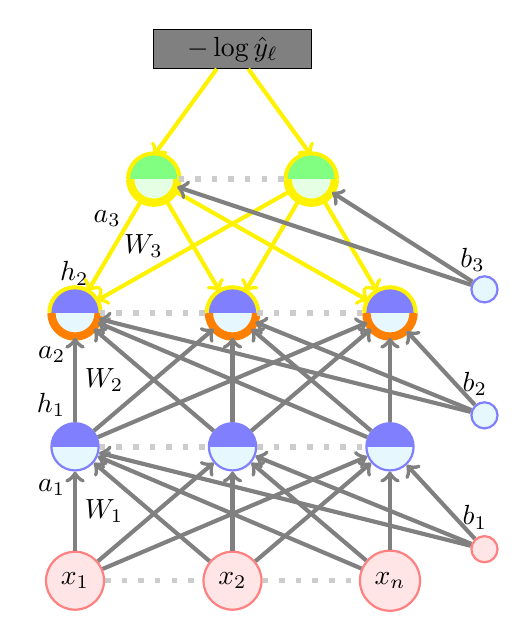
\begin{tikzpicture}
	\node [input_neuron] (neuron01) at (0,0) {$x_1$};
	\node [input_neuron] (neuron02) at (2,0){$x_2$};
	\node [input_neuron] (neuron03) at (4,0) {$x_n$};

	\node [bias_neuron] (neuron04) at (5.2,0.4) {};


	\node [hidden_neuron] (neuron11) at (0,1.7)  {};
	\node [hidden_neuron] (neuron12) at (2,1.7)  {};
	\node [hidden_neuron] (neuron13) at (4,1.7)  {};

	\node [bias_hidden_neuron] (neuron14) at (5.2,2.1) {};

	\begin{scope}
		\path[clip] (0,1.7) circle (3mm);
		\path[fill=blue!50] (-0.4,1.7) rectangle (0.3,2);
	\end{scope}
	\begin{scope}
		\path[clip] (2,1.7) circle (3mm);
		\path[fill=blue!50] (1.6,1.7) rectangle (2.3,2);
	\end{scope}
	\begin{scope}
		\path[clip] (4,1.7) circle (3mm);
		\path[fill=blue!50] (3.6,1.7) rectangle (4.3,2);
	\end{scope}


	\node [hidden_neuron] (neuron21) at (0,3.4)  {};
	\node [hidden_neuron] (neuron22) at (2,3.4)  {};
	\node [hidden_neuron] (neuron23) at (4,3.4)  {};

	\draw [yellow, line width = 3] (0.3,3.4) arc (0:180:3mm) {};
	\draw [yellow, line width = 3] (2.3,3.4) arc (0:180:3mm) {};
	\draw [yellow, line width = 3] (4.3,3.4) arc (0:180:3mm) {};

	\draw[orange, line width = 3] (-0.3, 3.4) arc (180:360:3mm){};
	\draw[orange, line width = 3] (1.7, 3.4) arc (180:360:3mm){};
	\draw[orange, line width = 3] (3.7, 3.4) arc (180:360:3mm){};
	\node [bias_hidden_neuron] (neuron24) at (5.2,3.7) {};


	\begin{scope}
		\path[clip] (0,3.4) circle (3mm);
		\path[fill=blue!50] (-0.4,3.4) rectangle (0.4,3.7);
	\end{scope}
	\begin{scope}
		\path[clip] (2,3.4) circle (3mm);
		\path[fill=blue!50] (1.6,3.4) rectangle (2.4,3.7);
	\end{scope}
	\begin{scope}
		\path[clip] (4,3.4) circle (3mm);
		\path[fill=blue!50] (3.6,3.4) rectangle (4.4,3.7);
	\end{scope}


	\node [output_neuron] (neuron31) at (1,5.1)  {};
	\node [output_neuron] (neuron32) at (3,5.1)  {};
	\draw [fill=gray] (1, 7) rectangle (3, 6.5) node[pos=0.5] {$-\log\hat{y}_\ell$};
	%\draw [black!50,line width=1.5pt,  ->] (1, 5.4) -- (1.8, 6.5);
	%\draw [black!50, line width=1.5pt, ->]  (3, 5.4) -- (2.2, 6.5);
	\draw [yellow,line width=1.5pt,  ->] (1.8, 6.5) -- (1, 5.4);
	\draw [yellow, line width=1.5pt, ->]  (2.2, 6.5) -- (3, 5.4);
	\draw [yellow, line width = 3] (1.3,5.1) arc (0:180:3mm) {};
	\draw [yellow, line width = 3] (3.3,5.1) arc (0:180:3mm) {};
	\draw[yellow, line width = 3] (0.7, 5.1) arc (180:360:3mm){};
	\draw[yellow, line width = 3] (2.7, 5.1) arc (180:360:3mm){};


	\begin{scope}
		\path[clip] (1,5.1) circle (3mm);
		\path[fill=green!50] (0.6,5.1) rectangle (1.3,5.4);
	\end{scope}
	\begin{scope}
		\path[clip] (3,5.1) circle (3mm);
		\path[fill=green!50] (2.6,5.1) rectangle (3.3,5.4);
	\end{scope}

	\draw[white,->] (neuron01) -- (neuron11) node[black,pos=.5,right]  {$W_{1}$} node[black,pos=0.8,left] {$a_{1}$};

	\draw[white,->] (neuron11) -- (neuron21) node[black,pos=.5,right] {$W_{2}$} node[black,pos=0.8,left] {$a_{2}$} node[black,pos=.2,left] {$h_{1}$};
	\draw[white,->] (neuron21) -- (neuron31) node[black,pos=.5,right] {$W_{3}$} node[black,pos=0.8,left] {$a_{3}$} node[black,pos=.2,left] {$h_{2}$};

	\draw[white,->] (neuron04) -- (neuron13) node[black,pos=0,right,above] {$b_1$};

	\draw[white,->] (neuron14) -- (neuron23) node[black,pos=0,right,above] {$b_2$};

	\draw[white,->] (neuron24) -- (neuron32) node[black,pos=0,right,above] {$b_3$};


	%\draw[white,->] (neuron31) -- (2.4.9) node[black,pos=1,above] {y };
	%\draw[white,->] (neuron31) -- (3,6.5) node[black,pos=1,above] {$f(x)$};
	%node[pos=1.3,above,right] {$\mathscr{L}(\theta)$};

	\draw[black!20,line width=2pt,loosely dotted] (neuron01) -- (neuron02);
	\draw[black!20,line width=2pt,loosely dotted] (neuron02) -- (neuron03);
	\draw[black!20,line width=2pt,loosely dotted] (neuron11) -- (neuron12);
	\draw[black!20,line width=2pt,loosely dotted] (neuron12) -- (neuron13);
	\draw[black!20,line width=2pt,loosely dotted] (neuron21) -- (neuron22);
	\draw[black!20,line width=2pt,loosely dotted] (neuron22) -- (neuron23);
	\draw[black!20,line width=2pt,loosely dotted] (neuron31) -- (neuron32);


	\foreach \from in {neuron01,neuron02,neuron03,neuron04}
	\foreach \to in {neuron11,neuron12,neuron13}
	\draw [black!50,line width=1.5pt,->] (\from) -- (\to);

	\foreach \from in {neuron11,neuron12,neuron13,neuron14}
	\foreach \to in {neuron21,neuron22,neuron23}
	\draw [black!50,line width=1.5pt,->] (\from) -- (\to);

	\foreach \from in {neuron21,neuron22,neuron23}
	\foreach \to in {neuron31,neuron32}
	\draw [yellow,line width=1.5pt,->] (\to) -- (\from);

	\draw [black!50,line width=1.5pt,->] (neuron24) -- (neuron31);
	\draw [black!50,line width=1.5pt,->] (neuron24) -- (neuron32);

\end{tikzpicture}

  \end{columns}
\end{frame}
